%!TEX root = ../main.tex
\section{Experiments}
\label{sec:experiments}
We started with defining a simple linear model as baseline and then created two  models
based on neural networks. In this section we explain the models' structure. Then the
setup of the  experiment will be described and in the end, we show the performance of our
models.

\subsection{The Baseline Model}
\label{subsec:experiments:baselinemodel}
We chose a linear regression model from scikit-learn \citep{scikit-learn} as our baseline. As
features we only used the categorical variables \emph{group}, \emph{post type} and \emph{top level 
domain}. The post types were already listed in section~\ref{subsec:dataset:description}.
The top level domain was extracted whenever a link was attached to the post. For the training 
dataset we ended up with 886 different top level domains. All categorical features were 
one-hot-encoded. The text of the post was omitted for the linear model.


\subsection{Neural Network based on DistilBert} 
\label{subsec:experiments:distilbertmodel}
The first model using neural networks was based on DistilBert \citep{sanh2020distilbert}.
We used the Python library \emph{transformers} \citep{wolf-etal-2020-transformers} which 
comes with a pre-trained tokenizer and vocabulary. The DistilBert model was used to
process text resulting from the concatenation of a post's \emph{message}, \emph{image text}, 
\emph{link text} and \emph{description}. In order to let the network process the categorical
features from section~\ref{subsec:experiments:baselinemodel} they were one-hot-encoded,
and then input in a one layer network.  The output of both was concatenated and finally
processed through a linear layer with the output size of one. Only rectified linear units
were used as non linearities. Adam~\citep{DBLP:journals/corr/KingmaB14} was used as
optimizer.

\subsection{BiLSTM based Model} 
\label{subsec:experiments:bilstmmodel}
The second neural model was based on a BiLSTM and used a similar structure to the
DistilBert one.  While the BiLSTM was responsible for the textual features, the
categorical ones were processed by a  one layer neural network followed by a concatenation
of the BiLSTM's output which  then was processed by a single linear layer. Adam~\citep{DBLP:journals/corr/KingmaB14} was used as the optimizer for this model as well.

\subsection{Experiment Setup}
\label{subsec:experiments:setup}
We used a 60-20-20 split for the train, validation and testset. The metric we used to 
measure the performance was the mean squared error (MSE). For the models based on neural
networks, we tried different learning rates manually. 

\subsection{Results}
\label{subsec:experiments:results}
\begin{table}[tb]
    \caption{mean squared error for all models and datasets}
    \label{tab:results-all}
    \centering

    \begin{tabular}{l|l|l}
    \hline

    \hline
    & \textbf{conspiracy theory groups} & \textbf{rtnews}\\
    \hline
    linear model & 6.68 & 177.51\\
    \hline
    DistilBert & 6.46 & 177.00\\
    \hline
    BiLSTM & 6.54 & 177.44\\
    \hline
    \end{tabular}
\end{table}
\begin{table}[tb]
    \caption{mean squared error for each group}
    \label{tab:result-mse-per-group}
    \centering
    \begin{tabular}{l|l|l|l}
        Group & Linear Model & DistilBert based & BiLSTM \\
        \hline
        \hline
        Galactic Federation of Light & 12.71 & 12.49 & 12.58\\
        Presence & 3.51 & 3.39 & 3.46\\
        The Real Flat Earth vs Globe Earth & 2.18 & 2.16 & 2.07\\
        Ancient Aliens (World Wide) & 2.08 & 1.90 & 1.94\\
        Vaccine Resistance Movement VRM Updates \dots & 5.43 & 5.24 & 5.47\\
        Chemtrails Global Skywatch & 7.10 & 7.00 & 6.99\\
        The League of Extraordinary Flat Earthers \dots & 1.22 & 0.84 & 0.95\\
        Awakening Code Community 1111 3333 4444 & 7.75 & 7.42 & 7.61\\
        THE WATCHERS & 2.21 & 2.01 & 2.12\\
        Aliens, UFOs, Anunnaki, Ancient aliens, \dots & 6.72 & 5.97 & 6.21\\
    \end{tabular}
\end{table}
The lowest error was achieved by the neural model based on DistilBert with an MSE of 6.46
for the conspiracy theory group dataset and an MSE of 177 for the rtnews dataset. The 
results can be found in Table~\ref{tab:results-all}. In
Table~\ref{tab:result-mse-per-group} the MSE was calculated on a per group basis for the
conspiracy theory group dataset. The lowest error was achieved for the \emph{The League of
Extraordinary Flat Earthers | Flat Earth SubGeniuses} group's posts using the DistilBert
model with an MSE of 0.84.
\begin{figure}[tb]
    \centering
    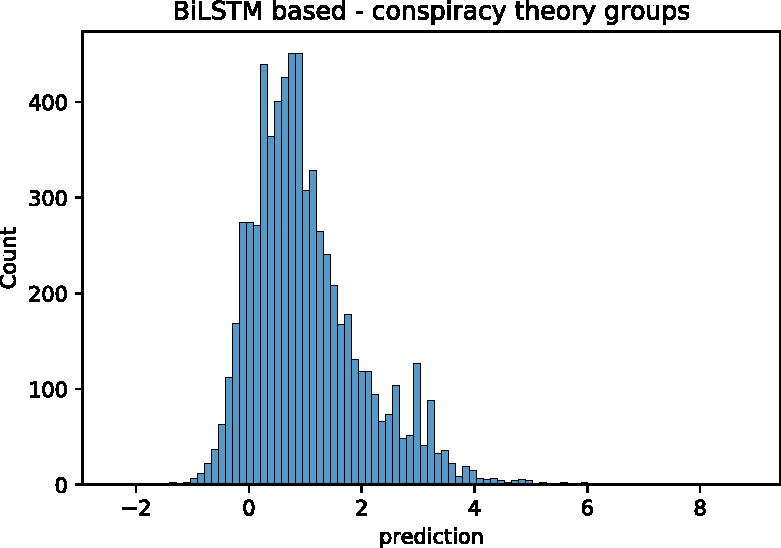
\includegraphics[width=.33\textwidth]{figures/prediction_groups/bilstm_dist.pdf}
    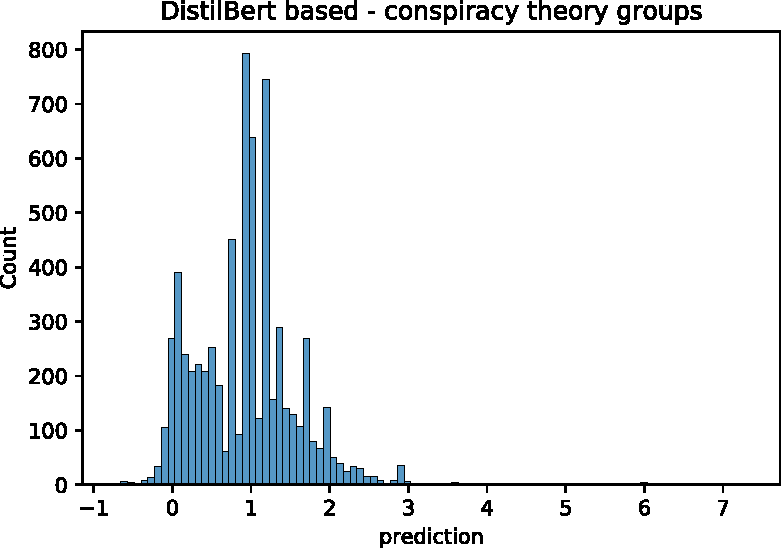
\includegraphics[width=.32\textwidth]{figures/prediction_groups/distil_bert_dist.pdf}
    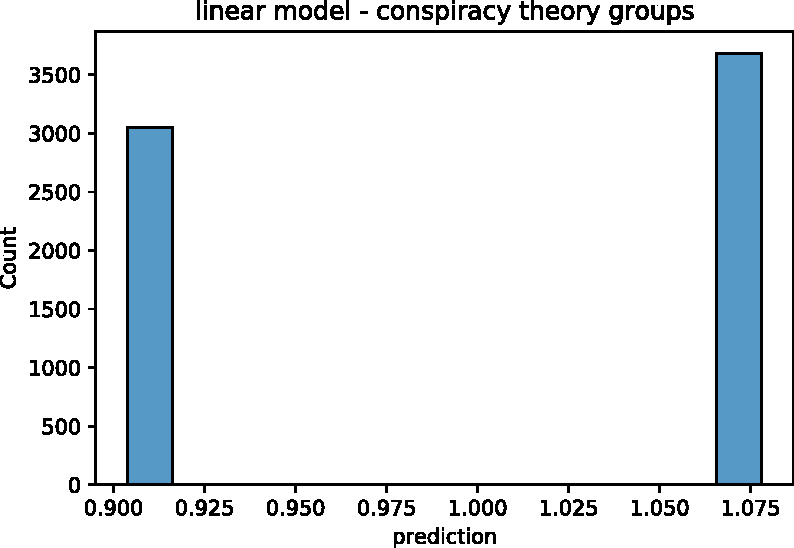
\includegraphics[width=.33\textwidth]{figures/prediction_groups/linear_model_prediction_dist.pdf}
    \caption{distribution of the model's score variable prediction for the conspiracy theory group dataset}
    \label{fig:dist-prediction-groups}
\end{figure}
\begin{figure}[tb]
    \centering
    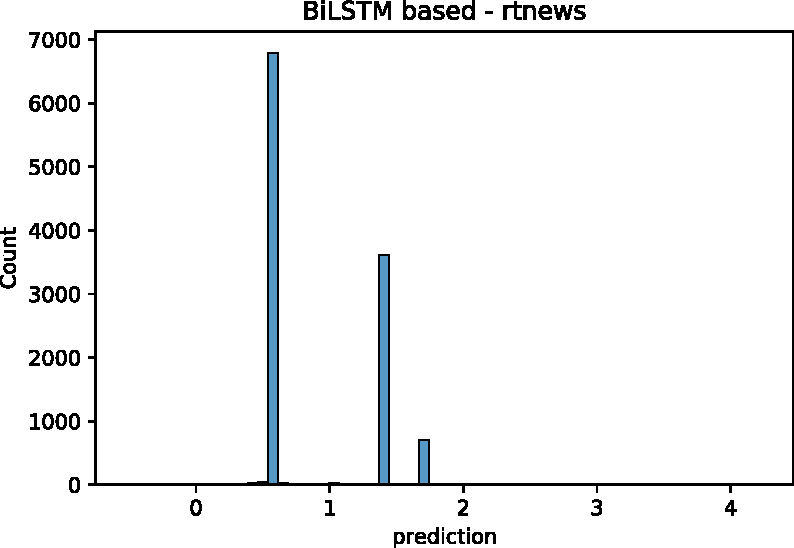
\includegraphics[width=.33\textwidth]{figures/prediction_rtnews/bilstm_dist.pdf}
    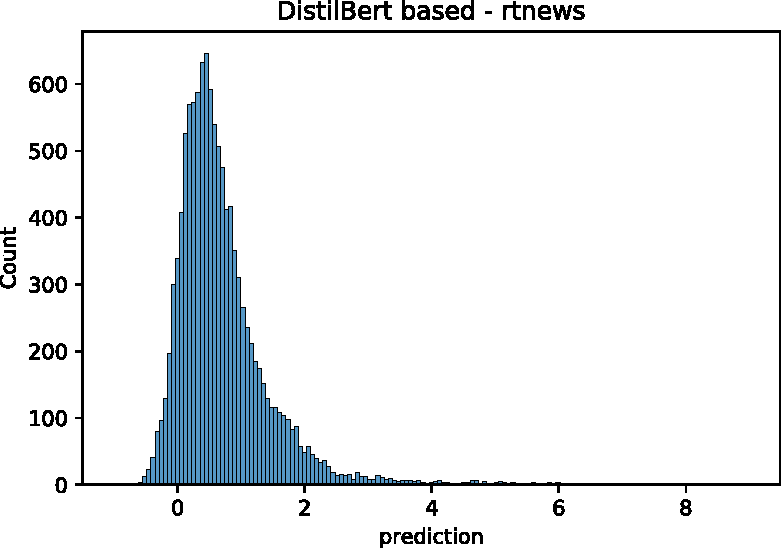
\includegraphics[width=.32\textwidth]{figures/prediction_rtnews/distil_bert_dist.pdf}
    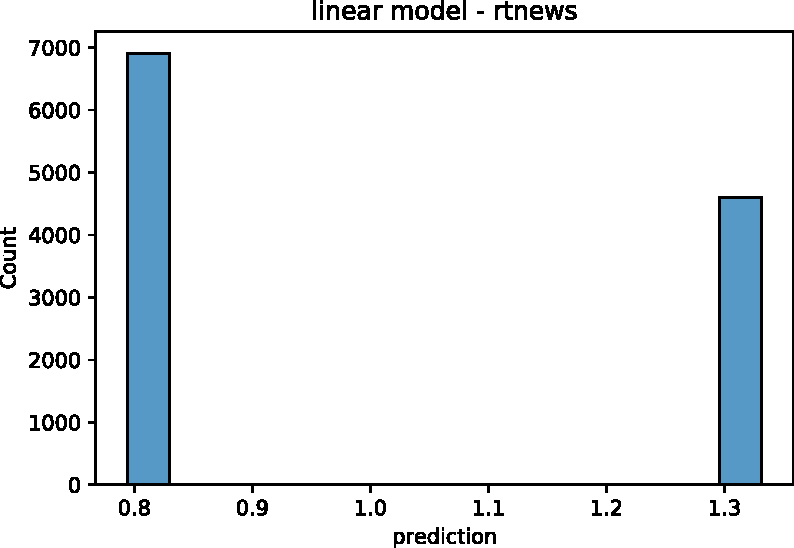
\includegraphics[width=.33\textwidth]{figures/prediction_rtnews/linear_model_prediction_dist.pdf}
    \caption{distribution of the model's score variable prediction for the rtnews dataset}
    \label{fig:dist-prediction-rtnews}
\end{figure}
The histograms of the models predictions can be seen in Figure~\ref{fig:dist-prediction-groups}
for the conspiracy theory group dataset and in Figure~\ref{fig:dist-prediction-rtnews} for 
the rtnews dataset. We assume that the linear model predicted an average based on one of 
the categorical variables (e.g. post type).